\section{Related Work}\label{sec:camrel}
Camera calibration is a well established method originating back to as early as the 1900s with lens research by Conrady~\cite{Conrady1919}. This developed into the Brown distortion model which forms the foundation for modern day camera calibration techniques~\cite{Brown1966,Brown1971,Brown1986}. One of the first openly available camera calibration tools was the Camera Calibration Toolbox for MATLAB. This tool, developed by Jean-Yves Bouguet, could calibrate a camera and return the intrinsic and extrinsic parameters. The toolbox was built on the foundation of work done by Tsai~\cite{Tsai1987} for introducing off the shelf technologies to camera calibration, Heikkila and Silven~\cite{Silven1997} for presenting an intrinsic calibration model, and most prominently Zhang for developing many of the techniques used in the toolbox~\cite{Zhang2000}. This work was later ported to OpenCV and used to develop the more powerful Computer Vision System Toolbox for MATLAB. These two tools are widely used in the field today. 

More complex calibration models have been developed to handle more complicated camera lenses taking into account different types of distortion. Specific methods to deal with extreme fisheye and barrel distortion have arose both in OpenCV and in independently released packages. Both the  Camera Calibration toolbox for MATLAB and OpenCV have a fisheye calibration model based on the work of Kannala and Brandt~\cite{Bradnt2006}. Scaramuzza have worked extensively with omnidirectional camera calibration and has developed his own MATLAB toolbox ~\cite{Scara2006_1,Scara2006_2,Scara2008_1,Scara2008_2}. Currently these are the state of the art readily available tools for rapid prototyping and used by the general public, each with its own advantages and disadvantages.

In recent years, there has been a push for the calibration of low cost and easily portable camera systems. With the development and continued advancement of products such as the GoPro, research has gone into the calibration and use of these cameras to solve imaging problems. Balletti et al. ~\cite{balletti2014calibration} explained many of the advantages of lightweight cameras including their ease to handle, capability of performing under extreme conditions, and providing high quality stills and video. They also explained methods for calibrating the cameras for reconstruction purposes. In the realm of underwater camera calibration, Schmidt and Rzhanov~\cite{schmidt2012measurement}, and Shortis~\cite{shortis2015calibration} compared the results and techniques for calibrating GoPro systems with the added distortion of water. These studies all fail to touch on the calibration of the GoPro camera when it is set to SuperView mode. 

\begin{figure}[t]
	\centering
	\fbox{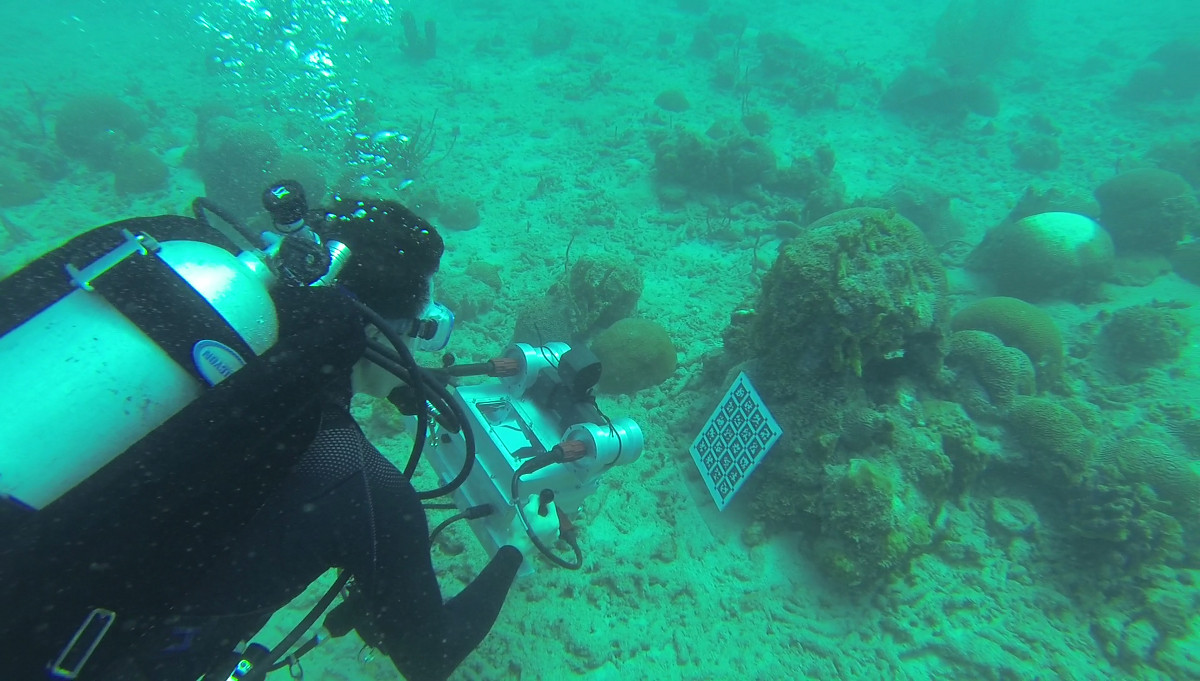
\includegraphics[width=0.9\textwidth]{figures/othersensors_red}}
	\caption{Diver calibrating an underwater rig consisting of stereo cameras and an IMU.}
	\label{fig:sensors}
\end{figure}

Calibration can be much more complicated and tedious if the camera is not the only sensor needing calibration. Many robotic systems take advantage of multiple proprioceptive and exteroceptive sensors in combination with visual input. A common proprioceptive sensor is the inertial measurement unit (IMU) which measures linear accelerations and angular velocities. Fig. \ref{fig:sensors} shows an example of the calibration process for a visual and interior sensor system. Significant efforts has been  in order to calibrate these systems as accurately as possible including the use of a Kalman Filter to determine the unknown coordinate transformations between sensors~\cite{4637877, doi:10.1177/0278364907079276, 2011_Kelly_Visual}. Because these calibrations rely heavily on the camera input, it is important that the camera calibration output is as accurate as possible so it will not skew the calibration of the other sensors. 



A system for assisting novice users to collect images for calibration through a Graphical User Interface is proposed by Richardson et al.~\cite{richardson2013iros}. 

Hu and Kantor~\cite{hu2016icra} presented a greedy approach for selecting images so that they are uniformly distributed over different camera poses. Such a method considers a budget that encodes the maximum processing time allowed. A quality metric could be considered to improve the performance.